\section{Literature Review}
\label{Chap2}
Before influential research in the context of \ac{SC} is presented, we want to introduce a standardized notation. Therefore, without loss of generality, assume that panel data is observed for $j = 0,1,...,J$ panel units and that unit $j = 0$ is exposed to treatment at period $T_0$. The temporal ordering is thus as follows:
$$
\underbrace{1,2,..., T_0 -1}_{T_{pre}},  \underbrace{T_0, T_0 +1, ..., T}_{T_{post}},
$$
such that $T_0 -1$ periods of pre-treatment data ($T_{pre}$) and $T-(T_0 -1)$ periods of post-treatment data ($T_{post}$) is observed.

\textit{Canonical Applications}\\
In their canonical 2003 article, \cite{abadie:2003} evaluate the causal economic effects of conflict using terrorist conflicts in the Basque Country as a comparative case study. Their data consists of $T_{pre} = 15$ $(1955-1969)$ periods of pre-treatment and $T_{post} = 28$  $(1970-1997)$ periods of post-treatment data for $J = 16$ controls and the single treatment unit indexed by $j = 0$. By constructing a synthesized Basque country that is computed as a weighted average of  the remaining regions in Spain that did not experience terrorist conflicts, they invent the \ac{SC}-method to conduct causal inference in observational settings. The weights are computed such that they optimally match the central variable of interest (\ac{GDP} per capita) as well as a set of time-invariant covariates of the central outcome variable for the treatment unit in the pre-treatment period. Constraining the weights to be weakly positive and to sum up to one provides an easy-to-interpret percentage interpretation and ensures that the synthetic control generalizes well in the post-treatment period. They find that terrorist conflicts caused the per capita \ac{GDP} of the treatment unit (Basque Country) to decline by about 10\% relative to the synthesized control unit. \\
The estimation of a comprehensive anti-smoking legislation in California in 1988 constitutes another central application of the \ac{SC} method by \cite{abadie:2010}. Here, the outcome of interest is per capita smoking in California and 29 U.S. states without such tobacco control programs serve as control units, referred to as Donors. The authors build their estimation on only $T_{pre} = 18$ $(1970-1987)$ pre-treatment years of data and $T_{post} = 13$ $(1988-2000)$, indicating the necessity to employ alternatives to the inestimable \ac{OLS} estimator. \cite{abadie:2010} reckon that Proposition 99 had a substantial, time-increasing negative effect on per capita cigarette sales by an average of almost 20 packs per person (approximate decline of 25\%). Besides presenting the causal treatment effect, the scholars also investigate the statistical significance of their results. By applying a version of the Exact Hypothesis Test proposed by \cite{fisher:1971}, they find that the probability of experiencing a treatment effect as extreme as observed for California is only 2.6\%.\\
The reunification of East and West Germany correlated strongly with an observable slow-down of \ac{GDP} per capita growth in West Germany. \cite{abadie:2015} utilize this natural experiment as another application of the \ac{SC}-method. In contrast to other applications of \ac{SC}, the reunification-dataset is somewhat more wealthy as data is observed for $T_{pre} = 30$ $(1960-1989)$, $T_{post} = 14$ $(1990-2003)$ years and $J = 16$ donors and West Germany. From 1992 onward, they identify a clear negative average treatment effect of about \$1,600 per capita and year (approximately 8\% reduction compared to the 1990 baseline level). In order to examine the trade-off between interpretation and statistical optimality, they sequentially remove donor units from the synthetic control and re-estimate the model. In doing so, they find that the synthetic control heavily relies on one donor (Austria), a peculiarity arising from the specific restrictions (no intercept and percent-like coefficients) of the method.

\textit{Further Applications and Developments}\\
\cite{athey:2016} examine the topic of causal inference in observational studies at a higher level of abstraction and present their often quoted assessment of \ac{SC} being arguable "the most important innovation in policy innovation in the last 15 years". Besides elaborating on the synthetic control method, their work also includes a careful discussion of related methods for causal inference in observational studies such as regression discontinuity design, differences-in-differences, and particularly in context of high-dimensional settings, machine learning methods. \\
\cite{doudchenko:2016} specifically focus on the identifying assumptions of \ac{SC}. Besides the thorough treatment of the relationship between the amount of explanatory variables $J$ and pre-treatment observations $T_{pre}$, they focus in great detail on the four prevailing restrictions on the intercept and the weights, namely the no-intercept assumption, the adding-up and non-negativity assumption as well as the potential restriction of constant weights. Their main recommendation is to leave the restrictions aside and to opt for an elastic-net regression that ensures external validity by means of regularization. They apply the elastic together with three other proposal models to three core applications of \ac{SC} and obtain comparable results for the different models. \\
The \ac{SC}-method is also widely used in contemporary research: For example, \cite{born:2019} apply the method to quantify the economic cost of nationalism in context of the Brexit referendum vote and find that the so-called "doppelganger gap", i.e. the difference between actual and synthesized \ac{GDP}-trajectory of the \ac{UK} ranged between 1.7 and 2.5\% after \ac{UK}'s citizens voted against remaining in the EU. To disentangle their estimated treatment effect, the scholars proceed in two steps: First, by disassembling \ac{GDP} into its components, they find that consumption and investment are the main drivers of the decline. Second, they estimate an expectation-adjusted \ac{VAR}-model to explicitly account for anticipation and uncertainty. \\
Another recent synthetic control article was written by \cite{muhlbach:2019}. The authors study the causal effect of the relocation of the US embassy from Tel Aviv to Jerusalem on the weekly number of conflicts in Israel and Palestine. However, instead of relying on the conventional \ac{SC} method or related linear models, they opt for a random forest regression. They prove the asymptotic unbiasedness of the estimate as well as its consistency and conclude that their approach is not dominated by the remaining comparison models like the \ac{SC}. As expected, the relocation of the embassy caused an increase of conflicts. By conducting various inferences tests, the scholars find statistical significance at the 1\% level.\\
\cite{harvey:2020} pursue a multivariate structural time series approach to estimate the counterfactual for the treatment unit. Importantly, they argue that the decision for or against a potential donor should be made on the basis of stationarity tests and show such tests are applicable in small samples. They re-estimate two of the core \ac{SC} applications (tobacco control and German reunification) and conduct the KPSS-test for the difference between the treatment series and each potential donor to analyse stationary patterns. If the test rejects the null of stationarity around a deterministic trends, this serves as evidence against a balanced growth model and the potential donor should not be included in the counterfactual.\\
An incomplete list of recent \ac{SC} application also includes \cite{cho:2020} and  \cite{cunningham:2021}. Cho quantifies the impact of non-pharmaceutical interventions during the COVID-19 outbreak in Sweden and obtains robust indications for the adverse public health effects of tentative intervention policies during the COVID-19 pandemic. Cunningham studies the effect of incarceration in Texas on drug markets. Besides identifying only moderate effects of Texas doubling the state's prison capacities on the drug market, Cunningham has a salient point on the practical use of \ac{SC}: "Authors using synthetic control must do more than merely run the synth command when doing comparative case studies. They must find the exact p-values through placebo-based inference, check for the quality of the pre-treatment fit, investigate the balance of the covariates used for matching, and check for the validity of the model through placebo estimation [...]." \\
\cite{benmichael:2021a} connect to the commonly violated assumption of a perfect pre-treatment fit of the original \ac{SC} method: they introduce the augmented synthetic control method that accounts for a potential bias of the \ac{SC}-estimator due to imperfect pre-treatment fit. Simplified, their model uses a ridge penalty to improve the pre-treatment fit and penalizes extrapolation from the convex hull of the donors. In some applications, interventions are subject to staggered adoption, i.e. multiple panel units adopting a given given treatment at different times. \cite{benmichael:2021b} generalize the original \ac{SC}-method to such scenarios by proposing a "partially pooled" \ac{SC} that allows for unit-level intercepts and covariates. \\
Last but not least, \cite{abadie:2019} propose the so-called penalized synthetic control estimator that is closely related to staggered adoption. The development is motivated by the observation that the original \ac{SC} method is increasingly applied to settings of multiple treated units. In such contexts, the overall treatment effect can be approached through two distinct methodologies. The first entails aggregating all treatment units and subsequently calculating the synthetic control, whereas the second involves the computation of  synthetic controls for each unit, followed by the aggregation of these individual synthetic controls. Specifically when the matching variables for the treatment units fall inside the convex hull of the donor pool, nonuniqueness of the weights is likely to be a concern. To solve this issue, the authors provide a regularization that trades off the competing objectives of minimizing covariate discrepancy between each donor and its specific synthetic control and the objective of minimizing covariate discrepancy between each donor and the aggregated synthetic control.

\textit{Hypothesis Tesing}\\
The question of treatment effect significance arises naturally subsequent to the construction of the synthetic control. \ac{ADH} propose a model-invariant non-parametric inference procedure that is based on the Exact Hypothesis Test proposed by \cite{fisher:1971}. %\footnote{The basic idea behind such permutation tests is to compare the observed data with a number of randomly permuted versions of it, and to use the distribution of the test statistic calculated from the permutations to estimate the probability that the observed result occurred by chance.} 
\ac{ADH} consider permutations in region (i.e. panel unit) and time. Region permutations estimate the treatment effect for each panel unit $j \in \{0, ..., J \}$.\footnote{Note that it is necessary to exclude the truly treated unit from donor pool as otherwise, it will contaminate the synthetic control} This procedure provides the researcher with the empirical $(J+1)$-observational distribution of the treatment. Next, the estimated treatment effect of the truly treated unit can be compared to the $J$ placebo-treatment effects of the donors. Given the estimated treatment effect for the truly treated unit is large, the null hypothesis of no treatment effect can be rejected at the significance level of one minus the percentile of treatment effect in the empirical distribution.\footnote{For instance, let $J = 99$ such that treatment effects for 100 panel units can be computed. As long as the estimated treatment effect of the truly treated units belongs to the 95 most extreme effects (95th percentile or higher), the permutation test rejects the null hypothesis of no treatment effect at least at 5 percent.} Time permutations consider only the truly treated unit and permute the treatment to time periods prior to the true treatment date $T_0$. Given that $T_0 > J$, this approach can increase the sensitivity of the test, since the theoretically feasible significance threshold of region permutation tests is determined by $\frac{1}{J}$. For both, region and time permutations, \ac{ADH} condense the estimated treatment effects into a precision metric like the post-treatment \ac{MSE}. Outlier in the donor pool can cause problems: Suppose for instance, that one donor region is very different from the rest such that it falls outside the convex hull of the remaining donors.\footnote{Note, that this circumstance does not cause problems for the truly treated region and its synthesized counterfactual as we expect the \ac{SC}-algorithm to assign a near zero weight to such an outlier. } Since the outlier itself cannot be synthesized precisely by the donor pool, pre- and post-treatment \ac{MSE} are expected to be large. Consequently, the permutation test will be unreasonably conservative and \ac{ADH} propose to exclude regions that are hard to predict, i.e. who have a pre-treatment \ac{MSE} that exceeds the \ac{MSE} of the truly treated unit to a great extent. Figure \ref{F_01} visualizes the exclusion procedure in the tobacco control application of \ac{ADH}. 

\begin{figure}[H]
	\centering
	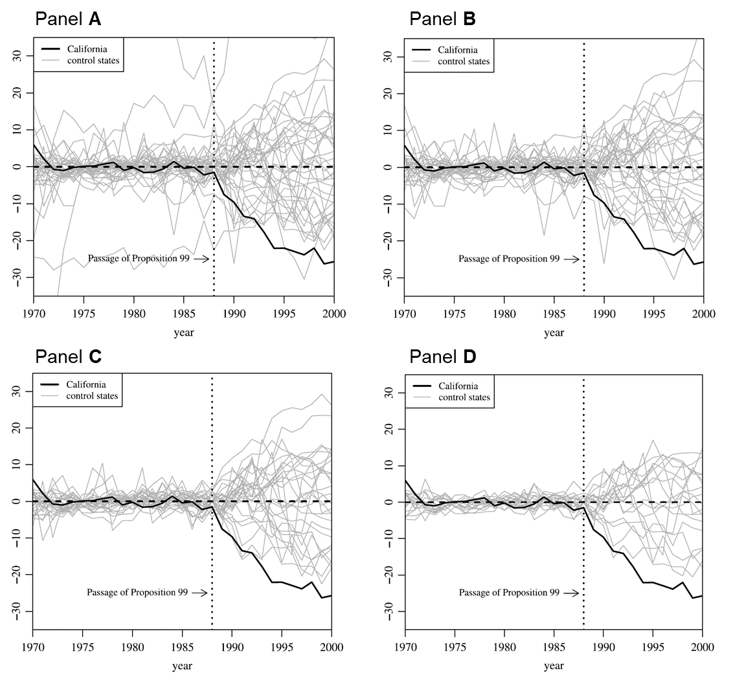
\includegraphics[scale=0.75]{F01}
	\caption{Region Exclusion Procedure of ADH}
	\label{F_01}
\end{figure}

The vertical axis indicates the gap between observed and estimated  per capita cigarette sales, the bold line represents the truly treated region (California). Some regions have both a poor pre- and post-treatment fit. Since the treatment significance should not be artificially driven by regions with poor fit, \ac{ADH} successively remove regions with a large pre-treatment \ac{MSE} relative to California. Panel B excludes regions with a \ac{MSE} that is more than 20 times as large the \ac{MSE} of California, Panel C lowers the cutoff to five times California's \ac{MSE} and Panel D to  two times the \ac{MSE}. In the last scenario, only 19 regions are left and California is the one with the most extreme treatment effect. The authors therefore conclude that the treatment is statistically significant with a (permutation) p-value of 5,3\% $\left(  \frac{1}{19} \right) $. One way to bypass the inefficient sample reduction procedure is to look at the distribution of the ratios of pre- and post-treatment \ac{MSE}. By scaling the post-treatment fit by the pre-treatment fit, regions with a poor fit are implicitly controlled for. In the tobacco control application, California is the region with the highest pre- to post-treatment \ac{MSE} ratio among all 39 regions, translating into a p-value of 2.6\% $\left(  \frac{1}{39} \right) $. \\
The end-of-sample test by \cite{andrews:2003} for structural breaks is another frequently applied econometric test to assess treatment effect significance. In comparison to the region  permutation test by \ac{ADH}, it does not rely on the assumption of random treatment. This distinction is crucial as 1) the random treatment assumption is unrealistic in many \ac{SC}  applications and 2) it does not require estimating the model for all units. Though the specific test statistic of the test is case specific, a commonly employed variant is based on the weighted sum of squared residuals. Under the null hypothesis of no structural break, this test statistic typically follows a known distribution like the standard normal and deviations indicate treatment effect significance. The test can be considered as a generalization of the F test by \cite{chow:1960}, allowing for more general error distributions than the one of the linear regression model.\\
\cite{chernozhukov:2021} take a similar perspective as \cite{andrews:2003} and interpret the causal inference problem as a counterfactual prediction task. Their test builds on the stochastic process of the time-specific difference between observed and synthesized outcome of the treatment unit. Under the null of no treatment effect, the pre- and post-treatment distribution of this processes should be indistinguishable. \cite{chernozhukov:2021} admit their tests relation to \cite{andrews:2003} end of sample test but highly important differences: First, they prove the high small sample performance of their test while Andrew's test relies on asymptotic analyses. Second, Andrews test assumes correct model specification, the test by Chernozhukov and colleagues is also valid under misspecification. Lastly, while Andrew's test is designed for low-dimensional models, their test generalizes well to high-dimensional models like tree-based estimators or neural nets. \\
Even in case the aforementioned tests hint toward general treatment effect significance, beyond some maximum forecast horizon, forecasts may become uninformative and volatile. \cite{breitung:2021} develop tests for the null hypothesis that forecasts from a survey of forecasters or from an estimated (parametric) model provide no more information than the unconditional mean of the series, i.e. that they become uninformative. In context of \ac{SC}, due to the fact that contemporaneous donor values are available over the entire post-treatment period, it is expected, that the null of uninformative forecasts is rejected at a significantly larger margin.
Independent of the specific test that is employed, prediction intervals should be computed to account for general forecasts uncertainty. For example, \cite{born:2019} define a prediction interval as plus minus one standard deviation of the pre-treatment prediction. If a normal approximation of the residuals seems reasonable, the 95\%-prediction interval would be comprised by plus minus 1.96 standard deviations of the pre-treatment prediction. Commonly, prediction intervals increase with the forecasts horizon to account for the fact that more uncertainty is associated with the forecast, the further ahead the forecast. Therefore, the naive standard deviation of a $h$-step forecast is usually given by $\hat{\sigma} \sqrt{h}$. Lastly, by means of bootstrapping of rejection sampling, the prediction interval could also be simulated. To bootstrap the prediction interval, one could draw e.g. $1,000$ observations with replacement from the data at hand, compute $1,000$ pre-treatment prediction standard deviations and define the 95\%-bootstrap prediction interval boundaries by the 25th and 975th largest standard deviation. To apply a rejection sampling approach, similar to Bayesian posterior sampling, one would generate a sample of, e.g. $1,000$ standard deviations obtained by the accept-and-reject cycle of the rejection sampling approach and define the prediction interval analogously to the bootstrap interval (see e.g. \cite{diebold:2017}, \cite{gebhard:2012} and \cite{koop:2003}).

%\cite{chernozhukov:2019} not read.\\
%\cite{firpo:2018} not read. \\
%\cite{hahn:2017} read.\\








